% https://fivethirtyeight.com/features/what-if-robots-cut-your-pizza/

\documentclass[varwidth, border = 40pt]{standalone}

\usepackage{tikz}
\usepackage{xcolor}

\definecolor{vdarkgray}{HTML}{1a1a1a}
\definecolor{vgray}{HTML}{686868}
\definecolor{vblue}{HTML}{007acc}


\begin{document}
	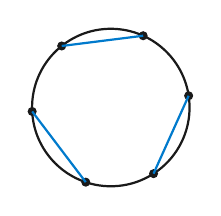
\begin{tikzpicture}
		\draw[color=vdarkgray, thick] (0,0) circle (1);
		\draw[color=vdarkgray, fill=vdarkgray] ({cos((.1 + pi / 3) r)},{sin((.1 + pi / 3) r)}) circle (.05);
		\draw[color=vdarkgray, fill=vdarkgray] ({cos((.15 + 2*pi / 3) r)},{sin((.15 + 2*pi / 3) r)}) circle (.05);
		\draw[color=vdarkgray, fill=vdarkgray] ({cos((.05 + 3*pi / 3) r)},{sin((.05 + 3*pi / 3) r)}) circle (.05);
		\draw[color=vdarkgray, fill=vdarkgray] ({cos((.2 + 4*pi / 3) r)},{sin((.2 + 4*pi / 3) r)}) circle (.05);
		\draw[color=vdarkgray, fill=vdarkgray] ({cos((.05 + 5*pi / 3) r)},{sin((.05 + 5*pi / 3) r)}) circle (.05);
		\draw[color=vdarkgray, fill=vdarkgray] ({cos((.15 + 6*pi / 3) r)},{sin((.15 + 6*pi / 3) r)}) circle (.05);
		\coordinate (A)	 at ({cos((.1 + pi / 3) r)},{sin((.1 + pi / 3) r)});
		\coordinate (B)	 at ({cos((.15 + 2*pi / 3) r)},{sin((.15 + 2*pi / 3) r)});
		\coordinate (C)	 at ({cos((.05 + 3*pi / 3) r)},{sin((.05 + 3*pi / 3) r)});
		\coordinate (D)	 at ({cos((.2 + 4*pi / 3) r)},{sin((.2 + 4*pi / 3) r)});
		\coordinate (E)	 at ({cos((.05 + 5*pi / 3) r)},{sin((.05 + 5*pi / 3) r)});
		\coordinate (F)	 at ({cos((.15 + 6*pi / 3) r)},{sin((.15 + 6*pi / 3) r)});
		\draw[color=vblue, thick] (A) -- (B);
		\draw[color=vblue, thick] (C) -- (D);
		\draw[color=vblue, thick] (E) -- (F);
	\end{tikzpicture}%
	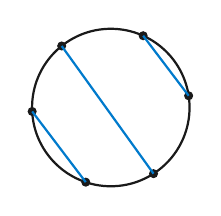
\begin{tikzpicture}
		\draw[color=vdarkgray, thick] (0,0) circle (1);
		\draw[color=vdarkgray, fill=vdarkgray] ({cos((.1 + pi / 3) r)},{sin((.1 + pi / 3) r)}) circle (.05);
		\draw[color=vdarkgray, fill=vdarkgray] ({cos((.15 + 2*pi / 3) r)},{sin((.15 + 2*pi / 3) r)}) circle (.05);
		\draw[color=vdarkgray, fill=vdarkgray] ({cos((.05 + 3*pi / 3) r)},{sin((.05 + 3*pi / 3) r)}) circle (.05);
		\draw[color=vdarkgray, fill=vdarkgray] ({cos((.2 + 4*pi / 3) r)},{sin((.2 + 4*pi / 3) r)}) circle (.05);
		\draw[color=vdarkgray, fill=vdarkgray] ({cos((.05 + 5*pi / 3) r)},{sin((.05 + 5*pi / 3) r)}) circle (.05);
		\draw[color=vdarkgray, fill=vdarkgray] ({cos((.15 + 6*pi / 3) r)},{sin((.15 + 6*pi / 3) r)}) circle (.05);
		\coordinate (A)	 at ({cos((.1 + pi / 3) r)},{sin((.1 + pi / 3) r)});
		\coordinate (B)	 at ({cos((.15 + 2*pi / 3) r)},{sin((.15 + 2*pi / 3) r)});
		\coordinate (C)	 at ({cos((.05 + 3*pi / 3) r)},{sin((.05 + 3*pi / 3) r)});
		\coordinate (D)	 at ({cos((.2 + 4*pi / 3) r)},{sin((.2 + 4*pi / 3) r)});
		\coordinate (E)	 at ({cos((.05 + 5*pi / 3) r)},{sin((.05 + 5*pi / 3) r)});
		\coordinate (F)	 at ({cos((.15 + 6*pi / 3) r)},{sin((.15 + 6*pi / 3) r)});
		\draw[color=vblue, thick] (A) -- (F);
		\draw[color=vblue, thick] (C) -- (D);
		\draw[color=vblue, thick] (E) -- (B);
	\end{tikzpicture}%
	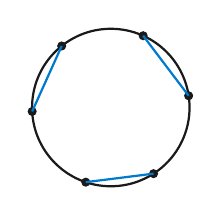
\begin{tikzpicture}
		\draw[color=vdarkgray, thick] (0,0) circle (1);
		\draw[color=vdarkgray, fill=vdarkgray] ({cos((.1 + pi / 3) r)},{sin((.1 + pi / 3) r)}) circle (.05);
		\draw[color=vdarkgray, fill=vdarkgray] ({cos((.15 + 2*pi / 3) r)},{sin((.15 + 2*pi / 3) r)}) circle (.05);
		\draw[color=vdarkgray, fill=vdarkgray] ({cos((.05 + 3*pi / 3) r)},{sin((.05 + 3*pi / 3) r)}) circle (.05);
		\draw[color=vdarkgray, fill=vdarkgray] ({cos((.2 + 4*pi / 3) r)},{sin((.2 + 4*pi / 3) r)}) circle (.05);
		\draw[color=vdarkgray, fill=vdarkgray] ({cos((.05 + 5*pi / 3) r)},{sin((.05 + 5*pi / 3) r)}) circle (.05);
		\draw[color=vdarkgray, fill=vdarkgray] ({cos((.15 + 6*pi / 3) r)},{sin((.15 + 6*pi / 3) r)}) circle (.05);
		\coordinate (A)	 at ({cos((.1 + pi / 3) r)},{sin((.1 + pi / 3) r)});
		\coordinate (B)	 at ({cos((.15 + 2*pi / 3) r)},{sin((.15 + 2*pi / 3) r)});
		\coordinate (C)	 at ({cos((.05 + 3*pi / 3) r)},{sin((.05 + 3*pi / 3) r)});
		\coordinate (D)	 at ({cos((.2 + 4*pi / 3) r)},{sin((.2 + 4*pi / 3) r)});
		\coordinate (E)	 at ({cos((.05 + 5*pi / 3) r)},{sin((.05 + 5*pi / 3) r)});
		\coordinate (F)	 at ({cos((.15 + 6*pi / 3) r)},{sin((.15 + 6*pi / 3) r)});
		\draw[color=vblue, thick] (A) -- (F);
		\draw[color=vblue, thick] (E) -- (D);
		\draw[color=vblue, thick] (B) -- (C);
	\end{tikzpicture}%
	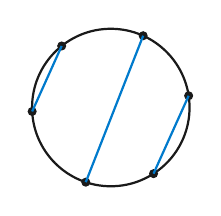
\begin{tikzpicture}
		\draw[color=vdarkgray, thick] (0,0) circle (1);
		\draw[color=vdarkgray, fill=vdarkgray] ({cos((.1 + pi / 3) r)},{sin((.1 + pi / 3) r)}) circle (.05);
		\draw[color=vdarkgray, fill=vdarkgray] ({cos((.15 + 2*pi / 3) r)},{sin((.15 + 2*pi / 3) r)}) circle (.05);
		\draw[color=vdarkgray, fill=vdarkgray] ({cos((.05 + 3*pi / 3) r)},{sin((.05 + 3*pi / 3) r)}) circle (.05);
		\draw[color=vdarkgray, fill=vdarkgray] ({cos((.2 + 4*pi / 3) r)},{sin((.2 + 4*pi / 3) r)}) circle (.05);
		\draw[color=vdarkgray, fill=vdarkgray] ({cos((.05 + 5*pi / 3) r)},{sin((.05 + 5*pi / 3) r)}) circle (.05);
		\draw[color=vdarkgray, fill=vdarkgray] ({cos((.15 + 6*pi / 3) r)},{sin((.15 + 6*pi / 3) r)}) circle (.05);
		\coordinate (A)	 at ({cos((.1 + pi / 3) r)},{sin((.1 + pi / 3) r)});
		\coordinate (B)	 at ({cos((.15 + 2*pi / 3) r)},{sin((.15 + 2*pi / 3) r)});
		\coordinate (C)	 at ({cos((.05 + 3*pi / 3) r)},{sin((.05 + 3*pi / 3) r)});
		\coordinate (D)	 at ({cos((.2 + 4*pi / 3) r)},{sin((.2 + 4*pi / 3) r)});
		\coordinate (E)	 at ({cos((.05 + 5*pi / 3) r)},{sin((.05 + 5*pi / 3) r)});
		\coordinate (F)	 at ({cos((.15 + 6*pi / 3) r)},{sin((.15 + 6*pi / 3) r)});
		\draw[color=vblue, thick] (A) -- (D);
		\draw[color=vblue, thick] (E) -- (F);
		\draw[color=vblue, thick] (B) -- (C);
	\end{tikzpicture}%
	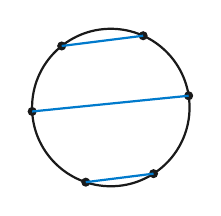
\begin{tikzpicture}
		\draw[color=vdarkgray, thick] (0,0) circle (1);
		\draw[color=vdarkgray, fill=vdarkgray] ({cos((.1 + pi / 3) r)},{sin((.1 + pi / 3) r)}) circle (.05);
		\draw[color=vdarkgray, fill=vdarkgray] ({cos((.15 + 2*pi / 3) r)},{sin((.15 + 2*pi / 3) r)}) circle (.05);
		\draw[color=vdarkgray, fill=vdarkgray] ({cos((.05 + 3*pi / 3) r)},{sin((.05 + 3*pi / 3) r)}) circle (.05);
		\draw[color=vdarkgray, fill=vdarkgray] ({cos((.2 + 4*pi / 3) r)},{sin((.2 + 4*pi / 3) r)}) circle (.05);
		\draw[color=vdarkgray, fill=vdarkgray] ({cos((.05 + 5*pi / 3) r)},{sin((.05 + 5*pi / 3) r)}) circle (.05);
		\draw[color=vdarkgray, fill=vdarkgray] ({cos((.15 + 6*pi / 3) r)},{sin((.15 + 6*pi / 3) r)}) circle (.05);
		\coordinate (A)	 at ({cos((.1 + pi / 3) r)},{sin((.1 + pi / 3) r)});
		\coordinate (B)	 at ({cos((.15 + 2*pi / 3) r)},{sin((.15 + 2*pi / 3) r)});
		\coordinate (C)	 at ({cos((.05 + 3*pi / 3) r)},{sin((.05 + 3*pi / 3) r)});
		\coordinate (D)	 at ({cos((.2 + 4*pi / 3) r)},{sin((.2 + 4*pi / 3) r)});
		\coordinate (E)	 at ({cos((.05 + 5*pi / 3) r)},{sin((.05 + 5*pi / 3) r)});
		\coordinate (F)	 at ({cos((.15 + 6*pi / 3) r)},{sin((.15 + 6*pi / 3) r)});
		\draw[color=vblue, thick] (E) -- (D);
		\draw[color=vblue, thick] (C) -- (F);
		\draw[color=vblue, thick] (B) -- (A);
	\end{tikzpicture}
	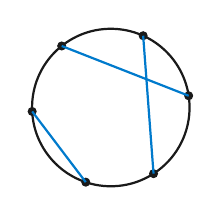
\begin{tikzpicture}
		\draw[color=vdarkgray, thick] (0,0) circle (1);
		\draw[color=vdarkgray, fill=vdarkgray] ({cos((.1 + pi / 3) r)},{sin((.1 + pi / 3) r)}) circle (.05);
		\draw[color=vdarkgray, fill=vdarkgray] ({cos((.15 + 2*pi / 3) r)},{sin((.15 + 2*pi / 3) r)}) circle (.05);
		\draw[color=vdarkgray, fill=vdarkgray] ({cos((.05 + 3*pi / 3) r)},{sin((.05 + 3*pi / 3) r)}) circle (.05);
		\draw[color=vdarkgray, fill=vdarkgray] ({cos((.2 + 4*pi / 3) r)},{sin((.2 + 4*pi / 3) r)}) circle (.05);
		\draw[color=vdarkgray, fill=vdarkgray] ({cos((.05 + 5*pi / 3) r)},{sin((.05 + 5*pi / 3) r)}) circle (.05);
		\draw[color=vdarkgray, fill=vdarkgray] ({cos((.15 + 6*pi / 3) r)},{sin((.15 + 6*pi / 3) r)}) circle (.05);
		\coordinate (A)	 at ({cos((.1 + pi / 3) r)},{sin((.1 + pi / 3) r)});
		\coordinate (B)	 at ({cos((.15 + 2*pi / 3) r)},{sin((.15 + 2*pi / 3) r)});
		\coordinate (C)	 at ({cos((.05 + 3*pi / 3) r)},{sin((.05 + 3*pi / 3) r)});
		\coordinate (D)	 at ({cos((.2 + 4*pi / 3) r)},{sin((.2 + 4*pi / 3) r)});
		\coordinate (E)	 at ({cos((.05 + 5*pi / 3) r)},{sin((.05 + 5*pi / 3) r)});
		\coordinate (F)	 at ({cos((.15 + 6*pi / 3) r)},{sin((.15 + 6*pi / 3) r)});
		\coordinate (F)	 at ({cos((.15 + 6*pi / 3) r)},{sin((.15 + 6*pi / 3) r)});
		\draw[color=vblue, thick] (C) -- (D);
		\draw[color=vblue, thick] (F) -- (B);
		\draw[color=vblue, thick] (A) -- (E);
	\end{tikzpicture}%
	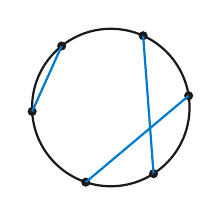
\begin{tikzpicture}
		\draw[color=vdarkgray, thick] (0,0) circle (1);
		\draw[color=vdarkgray, fill=vdarkgray] ({cos((.1 + pi / 3) r)},{sin((.1 + pi / 3) r)}) circle (.05);
		\draw[color=vdarkgray, fill=vdarkgray] ({cos((.15 + 2*pi / 3) r)},{sin((.15 + 2*pi / 3) r)}) circle (.05);
		\draw[color=vdarkgray, fill=vdarkgray] ({cos((.05 + 3*pi / 3) r)},{sin((.05 + 3*pi / 3) r)}) circle (.05);
		\draw[color=vdarkgray, fill=vdarkgray] ({cos((.2 + 4*pi / 3) r)},{sin((.2 + 4*pi / 3) r)}) circle (.05);
		\draw[color=vdarkgray, fill=vdarkgray] ({cos((.05 + 5*pi / 3) r)},{sin((.05 + 5*pi / 3) r)}) circle (.05);
		\draw[color=vdarkgray, fill=vdarkgray] ({cos((.15 + 6*pi / 3) r)},{sin((.15 + 6*pi / 3) r)}) circle (.05);
		\coordinate (A)	 at ({cos((.1 + pi / 3) r)},{sin((.1 + pi / 3) r)});
		\coordinate (B)	 at ({cos((.15 + 2*pi / 3) r)},{sin((.15 + 2*pi / 3) r)});
		\coordinate (C)	 at ({cos((.05 + 3*pi / 3) r)},{sin((.05 + 3*pi / 3) r)});
		\coordinate (D)	 at ({cos((.2 + 4*pi / 3) r)},{sin((.2 + 4*pi / 3) r)});
		\coordinate (E)	 at ({cos((.05 + 5*pi / 3) r)},{sin((.05 + 5*pi / 3) r)});
		\coordinate (F)	 at ({cos((.15 + 6*pi / 3) r)},{sin((.15 + 6*pi / 3) r)});
		\coordinate (F)	 at ({cos((.15 + 6*pi / 3) r)},{sin((.15 + 6*pi / 3) r)});
		\draw[color=vblue, thick] (C) -- (B);
		\draw[color=vblue, thick] (F) -- (D);
		\draw[color=vblue, thick] (A) -- (E);
	\end{tikzpicture}%
	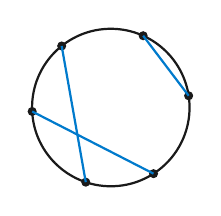
\begin{tikzpicture}
		\draw[color=vdarkgray, thick] (0,0) circle (1);
		\draw[color=vdarkgray, fill=vdarkgray] ({cos((.1 + pi / 3) r)},{sin((.1 + pi / 3) r)}) circle (.05);
		\draw[color=vdarkgray, fill=vdarkgray] ({cos((.15 + 2*pi / 3) r)},{sin((.15 + 2*pi / 3) r)}) circle (.05);
		\draw[color=vdarkgray, fill=vdarkgray] ({cos((.05 + 3*pi / 3) r)},{sin((.05 + 3*pi / 3) r)}) circle (.05);
		\draw[color=vdarkgray, fill=vdarkgray] ({cos((.2 + 4*pi / 3) r)},{sin((.2 + 4*pi / 3) r)}) circle (.05);
		\draw[color=vdarkgray, fill=vdarkgray] ({cos((.05 + 5*pi / 3) r)},{sin((.05 + 5*pi / 3) r)}) circle (.05);
		\draw[color=vdarkgray, fill=vdarkgray] ({cos((.15 + 6*pi / 3) r)},{sin((.15 + 6*pi / 3) r)}) circle (.05);
		\coordinate (A)	 at ({cos((.1 + pi / 3) r)},{sin((.1 + pi / 3) r)});
		\coordinate (B)	 at ({cos((.15 + 2*pi / 3) r)},{sin((.15 + 2*pi / 3) r)});
		\coordinate (C)	 at ({cos((.05 + 3*pi / 3) r)},{sin((.05 + 3*pi / 3) r)});
		\coordinate (D)	 at ({cos((.2 + 4*pi / 3) r)},{sin((.2 + 4*pi / 3) r)});
		\coordinate (E)	 at ({cos((.05 + 5*pi / 3) r)},{sin((.05 + 5*pi / 3) r)});
		\coordinate (F)	 at ({cos((.15 + 6*pi / 3) r)},{sin((.15 + 6*pi / 3) r)});
		\coordinate (F)	 at ({cos((.15 + 6*pi / 3) r)},{sin((.15 + 6*pi / 3) r)});
		\draw[color=vblue, thick] (C) -- (E);
		\draw[color=vblue, thick] (D) -- (B);
		\draw[color=vblue, thick] (A) -- (F);
	\end{tikzpicture}%
	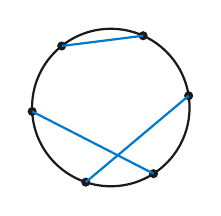
\begin{tikzpicture}
		\draw[color=vdarkgray, thick] (0,0) circle (1);
		\draw[color=vdarkgray, fill=vdarkgray] ({cos((.1 + pi / 3) r)},{sin((.1 + pi / 3) r)}) circle (.05);
		\draw[color=vdarkgray, fill=vdarkgray] ({cos((.15 + 2*pi / 3) r)},{sin((.15 + 2*pi / 3) r)}) circle (.05);
		\draw[color=vdarkgray, fill=vdarkgray] ({cos((.05 + 3*pi / 3) r)},{sin((.05 + 3*pi / 3) r)}) circle (.05);
		\draw[color=vdarkgray, fill=vdarkgray] ({cos((.2 + 4*pi / 3) r)},{sin((.2 + 4*pi / 3) r)}) circle (.05);
		\draw[color=vdarkgray, fill=vdarkgray] ({cos((.05 + 5*pi / 3) r)},{sin((.05 + 5*pi / 3) r)}) circle (.05);
		\draw[color=vdarkgray, fill=vdarkgray] ({cos((.15 + 6*pi / 3) r)},{sin((.15 + 6*pi / 3) r)}) circle (.05);
		\coordinate (A)	 at ({cos((.1 + pi / 3) r)},{sin((.1 + pi / 3) r)});
		\coordinate (B)	 at ({cos((.15 + 2*pi / 3) r)},{sin((.15 + 2*pi / 3) r)});
		\coordinate (C)	 at ({cos((.05 + 3*pi / 3) r)},{sin((.05 + 3*pi / 3) r)});
		\coordinate (D)	 at ({cos((.2 + 4*pi / 3) r)},{sin((.2 + 4*pi / 3) r)});
		\coordinate (E)	 at ({cos((.05 + 5*pi / 3) r)},{sin((.05 + 5*pi / 3) r)});
		\coordinate (F)	 at ({cos((.15 + 6*pi / 3) r)},{sin((.15 + 6*pi / 3) r)});
		\coordinate (F)	 at ({cos((.15 + 6*pi / 3) r)},{sin((.15 + 6*pi / 3) r)});
		\draw[color=vblue, thick] (C) -- (E);
		\draw[color=vblue, thick] (F) -- (D);
		\draw[color=vblue, thick] (A) -- (B);
	\end{tikzpicture}%
	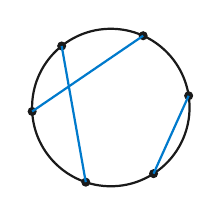
\begin{tikzpicture}
		\draw[color=vdarkgray, thick] (0,0) circle (1);
		\draw[color=vdarkgray, fill=vdarkgray] ({cos((.1 + pi / 3) r)},{sin((.1 + pi / 3) r)}) circle (.05);
		\draw[color=vdarkgray, fill=vdarkgray] ({cos((.15 + 2*pi / 3) r)},{sin((.15 + 2*pi / 3) r)}) circle (.05);
		\draw[color=vdarkgray, fill=vdarkgray] ({cos((.05 + 3*pi / 3) r)},{sin((.05 + 3*pi / 3) r)}) circle (.05);
		\draw[color=vdarkgray, fill=vdarkgray] ({cos((.2 + 4*pi / 3) r)},{sin((.2 + 4*pi / 3) r)}) circle (.05);
		\draw[color=vdarkgray, fill=vdarkgray] ({cos((.05 + 5*pi / 3) r)},{sin((.05 + 5*pi / 3) r)}) circle (.05);
		\draw[color=vdarkgray, fill=vdarkgray] ({cos((.15 + 6*pi / 3) r)},{sin((.15 + 6*pi / 3) r)}) circle (.05);
		\coordinate (A)	 at ({cos((.1 + pi / 3) r)},{sin((.1 + pi / 3) r)});
		\coordinate (B)	 at ({cos((.15 + 2*pi / 3) r)},{sin((.15 + 2*pi / 3) r)});
		\coordinate (C)	 at ({cos((.05 + 3*pi / 3) r)},{sin((.05 + 3*pi / 3) r)});
		\coordinate (D)	 at ({cos((.2 + 4*pi / 3) r)},{sin((.2 + 4*pi / 3) r)});
		\coordinate (E)	 at ({cos((.05 + 5*pi / 3) r)},{sin((.05 + 5*pi / 3) r)});
		\coordinate (F)	 at ({cos((.15 + 6*pi / 3) r)},{sin((.15 + 6*pi / 3) r)});
		\coordinate (F)	 at ({cos((.15 + 6*pi / 3) r)},{sin((.15 + 6*pi / 3) r)});
		\draw[color=vblue, thick] (D) -- (B);
		\draw[color=vblue, thick] (F) -- (E);
		\draw[color=vblue, thick] (A) -- (C);
	\end{tikzpicture}%
	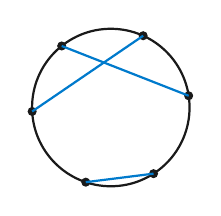
\begin{tikzpicture}
		\draw[color=vdarkgray, thick] (0,0) circle (1);
		\draw[color=vdarkgray, fill=vdarkgray] ({cos((.1 + pi / 3) r)},{sin((.1 + pi / 3) r)}) circle (.05);
		\draw[color=vdarkgray, fill=vdarkgray] ({cos((.15 + 2*pi / 3) r)},{sin((.15 + 2*pi / 3) r)}) circle (.05);
		\draw[color=vdarkgray, fill=vdarkgray] ({cos((.05 + 3*pi / 3) r)},{sin((.05 + 3*pi / 3) r)}) circle (.05);
		\draw[color=vdarkgray, fill=vdarkgray] ({cos((.2 + 4*pi / 3) r)},{sin((.2 + 4*pi / 3) r)}) circle (.05);
		\draw[color=vdarkgray, fill=vdarkgray] ({cos((.05 + 5*pi / 3) r)},{sin((.05 + 5*pi / 3) r)}) circle (.05);
		\draw[color=vdarkgray, fill=vdarkgray] ({cos((.15 + 6*pi / 3) r)},{sin((.15 + 6*pi / 3) r)}) circle (.05);
		\coordinate (A)	 at ({cos((.1 + pi / 3) r)},{sin((.1 + pi / 3) r)});
		\coordinate (B)	 at ({cos((.15 + 2*pi / 3) r)},{sin((.15 + 2*pi / 3) r)});
		\coordinate (C)	 at ({cos((.05 + 3*pi / 3) r)},{sin((.05 + 3*pi / 3) r)});
		\coordinate (D)	 at ({cos((.2 + 4*pi / 3) r)},{sin((.2 + 4*pi / 3) r)});
		\coordinate (E)	 at ({cos((.05 + 5*pi / 3) r)},{sin((.05 + 5*pi / 3) r)});
		\coordinate (F)	 at ({cos((.15 + 6*pi / 3) r)},{sin((.15 + 6*pi / 3) r)});
		\coordinate (F)	 at ({cos((.15 + 6*pi / 3) r)},{sin((.15 + 6*pi / 3) r)});
		\draw[color=vblue, thick] (E) -- (D);
		\draw[color=vblue, thick] (F) -- (B);
		\draw[color=vblue, thick] (A) -- (C);
	\end{tikzpicture}
	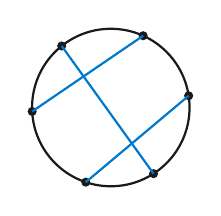
\begin{tikzpicture}
		\draw[color=vdarkgray, thick] (0,0) circle (1);
		\draw[color=vdarkgray, fill=vdarkgray] ({cos((.1 + pi / 3) r)},{sin((.1 + pi / 3) r)}) circle (.05);
		\draw[color=vdarkgray, fill=vdarkgray] ({cos((.15 + 2*pi / 3) r)},{sin((.15 + 2*pi / 3) r)}) circle (.05);
		\draw[color=vdarkgray, fill=vdarkgray] ({cos((.05 + 3*pi / 3) r)},{sin((.05 + 3*pi / 3) r)}) circle (.05);
		\draw[color=vdarkgray, fill=vdarkgray] ({cos((.2 + 4*pi / 3) r)},{sin((.2 + 4*pi / 3) r)}) circle (.05);
		\draw[color=vdarkgray, fill=vdarkgray] ({cos((.05 + 5*pi / 3) r)},{sin((.05 + 5*pi / 3) r)}) circle (.05);
		\draw[color=vdarkgray, fill=vdarkgray] ({cos((.15 + 6*pi / 3) r)},{sin((.15 + 6*pi / 3) r)}) circle (.05);
		\coordinate (A)	 at ({cos((.1 + pi / 3) r)},{sin((.1 + pi / 3) r)});
		\coordinate (B)	 at ({cos((.15 + 2*pi / 3) r)},{sin((.15 + 2*pi / 3) r)});
		\coordinate (C)	 at ({cos((.05 + 3*pi / 3) r)},{sin((.05 + 3*pi / 3) r)});
		\coordinate (D)	 at ({cos((.2 + 4*pi / 3) r)},{sin((.2 + 4*pi / 3) r)});
		\coordinate (E)	 at ({cos((.05 + 5*pi / 3) r)},{sin((.05 + 5*pi / 3) r)});
		\coordinate (F)	 at ({cos((.15 + 6*pi / 3) r)},{sin((.15 + 6*pi / 3) r)});
		\coordinate (F)	 at ({cos((.15 + 6*pi / 3) r)},{sin((.15 + 6*pi / 3) r)});
		\draw[color=vblue, thick] (C) -- (A);
		\draw[color=vblue, thick] (E) -- (B);
		\draw[color=vblue, thick] (F) -- (D);
	\end{tikzpicture}%
	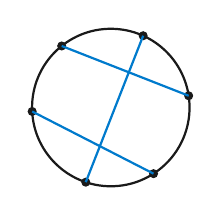
\begin{tikzpicture}
		\draw[color=vdarkgray, thick] (0,0) circle (1);
		\draw[color=vdarkgray, fill=vdarkgray] ({cos((.1 + pi / 3) r)},{sin((.1 + pi / 3) r)}) circle (.05);
		\draw[color=vdarkgray, fill=vdarkgray] ({cos((.15 + 2*pi / 3) r)},{sin((.15 + 2*pi / 3) r)}) circle (.05);
		\draw[color=vdarkgray, fill=vdarkgray] ({cos((.05 + 3*pi / 3) r)},{sin((.05 + 3*pi / 3) r)}) circle (.05);
		\draw[color=vdarkgray, fill=vdarkgray] ({cos((.2 + 4*pi / 3) r)},{sin((.2 + 4*pi / 3) r)}) circle (.05);
		\draw[color=vdarkgray, fill=vdarkgray] ({cos((.05 + 5*pi / 3) r)},{sin((.05 + 5*pi / 3) r)}) circle (.05);
		\draw[color=vdarkgray, fill=vdarkgray] ({cos((.15 + 6*pi / 3) r)},{sin((.15 + 6*pi / 3) r)}) circle (.05);
		\coordinate (A)	 at ({cos((.1 + pi / 3) r)},{sin((.1 + pi / 3) r)});
		\coordinate (B)	 at ({cos((.15 + 2*pi / 3) r)},{sin((.15 + 2*pi / 3) r)});
		\coordinate (C)	 at ({cos((.05 + 3*pi / 3) r)},{sin((.05 + 3*pi / 3) r)});
		\coordinate (D)	 at ({cos((.2 + 4*pi / 3) r)},{sin((.2 + 4*pi / 3) r)});
		\coordinate (E)	 at ({cos((.05 + 5*pi / 3) r)},{sin((.05 + 5*pi / 3) r)});
		\coordinate (F)	 at ({cos((.15 + 6*pi / 3) r)},{sin((.15 + 6*pi / 3) r)});
		\coordinate (F)	 at ({cos((.15 + 6*pi / 3) r)},{sin((.15 + 6*pi / 3) r)});
		\draw[color=vblue, thick] (D) -- (A);
		\draw[color=vblue, thick] (E) -- (C);
		\draw[color=vblue, thick] (F) -- (B);
	\end{tikzpicture}%
	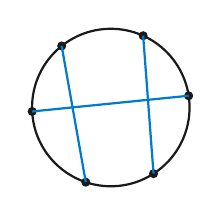
\begin{tikzpicture}
		\draw[color=vdarkgray, thick] (0,0) circle (1);
		\draw[color=vdarkgray, fill=vdarkgray] ({cos((.1 + pi / 3) r)},{sin((.1 + pi / 3) r)}) circle (.05);
		\draw[color=vdarkgray, fill=vdarkgray] ({cos((.15 + 2*pi / 3) r)},{sin((.15 + 2*pi / 3) r)}) circle (.05);
		\draw[color=vdarkgray, fill=vdarkgray] ({cos((.05 + 3*pi / 3) r)},{sin((.05 + 3*pi / 3) r)}) circle (.05);
		\draw[color=vdarkgray, fill=vdarkgray] ({cos((.2 + 4*pi / 3) r)},{sin((.2 + 4*pi / 3) r)}) circle (.05);
		\draw[color=vdarkgray, fill=vdarkgray] ({cos((.05 + 5*pi / 3) r)},{sin((.05 + 5*pi / 3) r)}) circle (.05);
		\draw[color=vdarkgray, fill=vdarkgray] ({cos((.15 + 6*pi / 3) r)},{sin((.15 + 6*pi / 3) r)}) circle (.05);
		\coordinate (A)	 at ({cos((.1 + pi / 3) r)},{sin((.1 + pi / 3) r)});
		\coordinate (B)	 at ({cos((.15 + 2*pi / 3) r)},{sin((.15 + 2*pi / 3) r)});
		\coordinate (C)	 at ({cos((.05 + 3*pi / 3) r)},{sin((.05 + 3*pi / 3) r)});
		\coordinate (D)	 at ({cos((.2 + 4*pi / 3) r)},{sin((.2 + 4*pi / 3) r)});
		\coordinate (E)	 at ({cos((.05 + 5*pi / 3) r)},{sin((.05 + 5*pi / 3) r)});
		\coordinate (F)	 at ({cos((.15 + 6*pi / 3) r)},{sin((.15 + 6*pi / 3) r)});
		\coordinate (F)	 at ({cos((.15 + 6*pi / 3) r)},{sin((.15 + 6*pi / 3) r)});
		\draw[color=vblue, thick] (C) -- (F);
		\draw[color=vblue, thick] (D) -- (B);
		\draw[color=vblue, thick] (A) -- (E);
	\end{tikzpicture}\\
	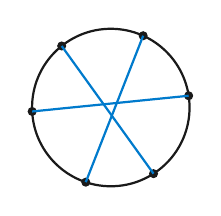
\begin{tikzpicture}
		\draw[color=vdarkgray, thick] (0,0) circle (1);
		\draw[color=vdarkgray, fill=vdarkgray] ({cos((.1 + pi / 3) r)},{sin((.1 + pi / 3) r)}) circle (.05);
		\draw[color=vdarkgray, fill=vdarkgray] ({cos((.15 + 2*pi / 3) r)},{sin((.15 + 2*pi / 3) r)}) circle (.05);
		\draw[color=vdarkgray, fill=vdarkgray] ({cos((.05 + 3*pi / 3) r)},{sin((.05 + 3*pi / 3) r)}) circle (.05);
		\draw[color=vdarkgray, fill=vdarkgray] ({cos((.2 + 4*pi / 3) r)},{sin((.2 + 4*pi / 3) r)}) circle (.05);
		\draw[color=vdarkgray, fill=vdarkgray] ({cos((.05 + 5*pi / 3) r)},{sin((.05 + 5*pi / 3) r)}) circle (.05);
		\draw[color=vdarkgray, fill=vdarkgray] ({cos((.15 + 6*pi / 3) r)},{sin((.15 + 6*pi / 3) r)}) circle (.05);
		\coordinate (A)	 at ({cos((.1 + pi / 3) r)},{sin((.1 + pi / 3) r)});
		\coordinate (B)	 at ({cos((.15 + 2*pi / 3) r)},{sin((.15 + 2*pi / 3) r)});
		\coordinate (C)	 at ({cos((.05 + 3*pi / 3) r)},{sin((.05 + 3*pi / 3) r)});
		\coordinate (D)	 at ({cos((.2 + 4*pi / 3) r)},{sin((.2 + 4*pi / 3) r)});
		\coordinate (E)	 at ({cos((.05 + 5*pi / 3) r)},{sin((.05 + 5*pi / 3) r)});
		\coordinate (F)	 at ({cos((.15 + 6*pi / 3) r)},{sin((.15 + 6*pi / 3) r)});
		\coordinate (F)	 at ({cos((.15 + 6*pi / 3) r)},{sin((.15 + 6*pi / 3) r)});
		\draw[color=vblue, thick] (C) -- (F);
		\draw[color=vblue, thick] (E) -- (B);
		\draw[color=vblue, thick] (A) -- (D);
	\end{tikzpicture}




\end{document}
